\section{Limits on New Physics}
\label{sec:limit}

%As discussed in Section~\ref{sec:results}, we see one event 
%in the signal region.
%The background prediction from the SM MC is 
%1.3 events.
%The data driven background predictions from the ABCD method 
%and the $\pt(\ell\ell)$ method are $1.3 \pm 0.8({\rm stat}) \pm 0.3({\rm syst})$ and
%$2.1 \pm 2.1({\rm stat}) \pm 0.6({\rm syst})$ events, respectively.

%These three predictions are in good agreement with each other
%and with the observation of one event in the signal region.
%We calculate a Bayesian 95\% CL upper limit~\cite{ref:cl95cms} 
%on the number of non SM events in the signal region to be 4.1,
%using a background prediction of $N_\textrm{BG}=1.4 \pm 0.8$
%events and a Gaussian model of nuissance parameter integration.  
%The upper limit is not very sensitive to $N_\textrm{BG}$ and its uncertainty.


The three background predictions for the high-\pt\ lepton trigger search
discussed in Section~\ref{sec:results} are in good agreement with each other and
with the observation of one event in the signal region. 
A Bayesian 95\%~confidence level (CL) upper limit~\cite{ref:cl95cms}  on the number of
non-SM events in the signal region is determined to be 4.0,
using a background prediction of $N_\textrm{BG} = 1.4 \pm 0.8$
events and a log-normal model of nuisance parameter integration.
The upper limit is not very sensitive to $N_\textrm{BG}$ and its uncertainty.
This generic upper limit is not corrected for the possibility
of signal contamination in the control regions. This is justified because
the two independent background estimation methods based on data agree
and are also consistent with the SM MC prediction.
Moreover,  no evidence for non-SM contributions in
the control regions is observed (Table~\ref{tab:datayield} and Figure~\ref{fig:victory}). 
This bound rules out the benchmark SUSY scenario LM0, for which the
number of expected signal events is $8.6 \pm 1.6$, while the LM1 scenario predicts
$3.6 \pm 0.5$ events.
The uncertainties in the LM0 and LM1 event yields arise from energy scale, luminosity, 
and lepton efficiency, as discussed in Section~\ref{sec:systematics}.

For the same-flavour search using hadronic activity triggers discussed in Section~\ref{sec:HT}, 
no same-flavour events are observed and the corresponding Bayesian 95\% CL upper limit on the 
non-SM yield is 3.0 events. 
This bound rules out the benchmark SUSY scenarios LM0 and LM1, for which the
numbers of expected signal events are $7.3 \pm 1.6$ and $3.6 \pm 0.7$, respectively.

%As an example of the sensitivity of this search, we 
%remind the reader that the number of expected signal events in the benchmark 
%SUSY scenarios LM0 and LM1 are $8.6 \pm 1.6$ and $3.6 \pm 0.5$, respectively, 
%where the uncertainties are from energy scale, luminosity, and lepton efficiency.


%Following text on CMSSM scan taken from RA1 paper
We also quote the result more generally in the context of the CMSSM.
The Bayesian 95\% CL limit  in the  $(m_0,m_{1/2})$ plane,  for $\tan\beta=3$,
$A_0 = 0$ and $\mu > 0$ is shown in Figure~\ref{fig:msugra}. 
The high-\pt\ lepton and hadronic trigger searches have similar sensitivity to the CMSSM; 
here we choose to show results based on the high-\pt\ lepton trigger search. The
SUSY particle  spectrum is calculated using  SoftSUSY~\cite{Allanach:2002uq}, and the
signal  events  are  generated  at  leading  order  (LO)  with  \PYTHIA6.4.22.
NLO  cross sections,  obtained  with the
program  Prospino~\cite{Beenakker:1997kx},  are used  to  calculate  the observed
exclusion  contour.  
At each point in the  $(m_0,m_{1/2})$ plane, the acceptance uncertainty is calculated by
summing in quadrature the uncertainties from jet and \MET\ energy scale using the
procedure discussed in Section~\ref{sec:systematics}, the uncertainty in the 
NLO cross section due to the choice of factorization and renormalization scale, 
and the uncertainty from the parton distribution function (PDF) for CTEQ6.6~\cite{Nadolsky:2008fk},
estimated from  the  envelope  provided  by  the  CTEQ6.6  error sets.
The luminosity uncertainty and dilepton
selection efficiency uncertainty are also included, giving a total relative acceptance uncertainty which varies
in the range 0.2--0.3.
%We consider a point excluded if the NLO yield exceeds the 95\% CL Bayesian upper limit
%calculated with this acceptance uncertainty, using a log-normal model for the nuisance
%parameter integration.
A point is considered to be excluded if the NLO yield exceeds the 95\% CL
Bayesian upper limit calculated with this acceptance uncertainty, using
a log-normal model for the nuisance parameter integration.
The limit curves do not include the effect of signal
contamination in the control regions.  We have verified that this
has a negligible impact on the excluded regions in Figure~\ref{fig:msugra}.

\begin{figure}[tbh]
\begin{center}
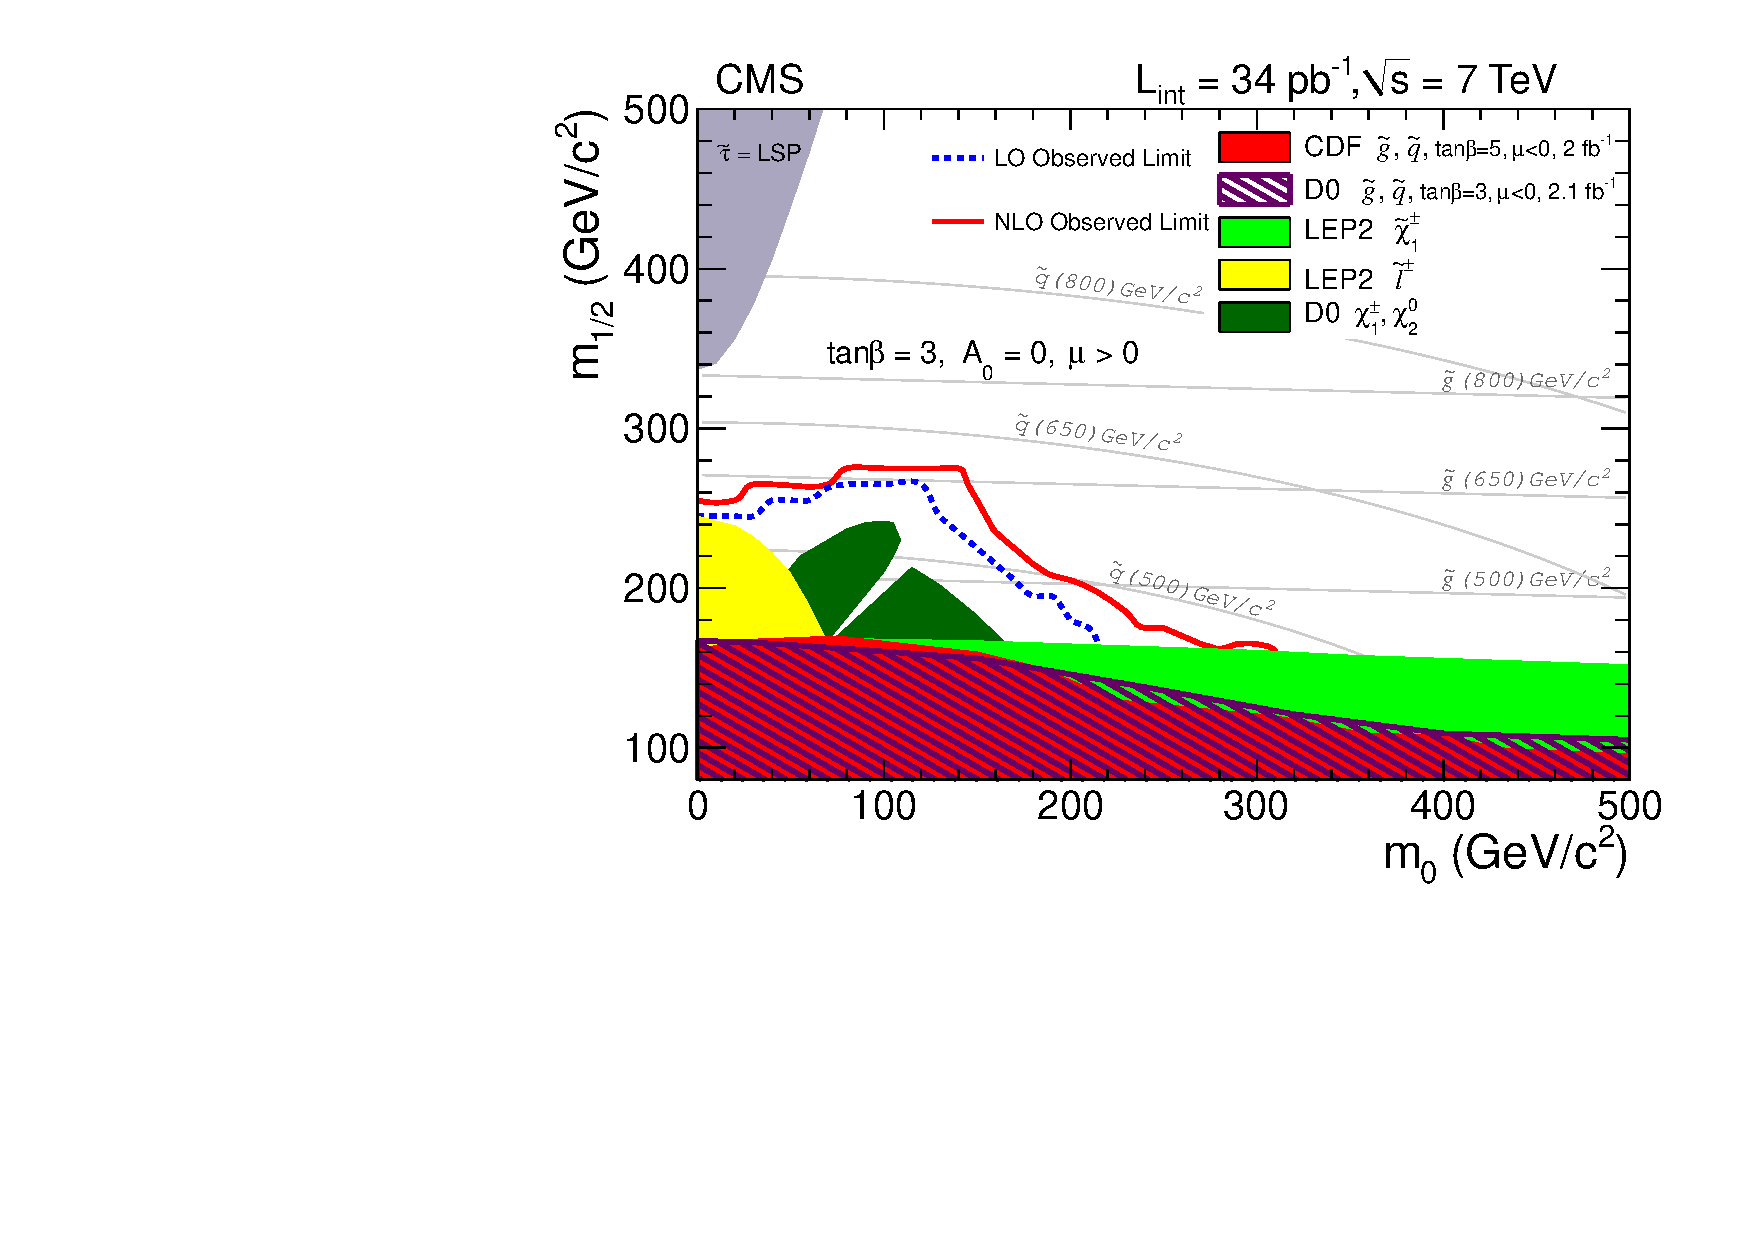
\includegraphics[width=1\linewidth]{plots_final/RA6_ExclusionLimit_tanb3_LO.pdf}
\caption{\label{fig:msugra}\protect 
%Text taken from RA1 paper
The observed 95\% CL exclusion contour at NLO (solid red line) and LO (dashed blue line) 
in the CMSSM $(m_0,m_{1/2})$ plane for  $\tan\beta=3$, $A_0 = 0$ and $\mu > 0$. 
The area below the curve is excluded by this measurement. Exclusion limits obtained from 
previous experiments are presented as filled areas in the plot. Thin grey lines correspond to 
constant squark and gluino masses.
%The plot also shows the two benchmark points LM0 and LM1 for comparison.
%Exclusion curve in the CMSSM parameter space, 
%assuming $\tan\beta=3$, sign of $\mu = +$ and $A_{0}=0\GeVcc$. 
}
\end{center}
\end{figure}

The excluded regions  for the CDF
search for  jets + missing  energy final states~\cite{PhysRevLett.102.121801} were
obtained for $\tan\beta=5$, while those from D0~\cite{Abazov2008449} were obtained for 
$\tan\beta=3$, each with  approximately  2~fb$^{-1}$ of  data and for $\mu < 0$. 
The  LEP-excluded
regions  are based  on searches  for  sleptons and  charginos~\cite{LEPSUSY}.  
%A comparison of the exclusion limit for tan b = 3 to that for tan b = 10
%for fixed values of A0 =  0 and sign(m) > 0 indicates that
%the exclusion  reach is only weakly  dependent on the value  of tan b;
%the limit shifts  by less than 20\GeV  in m0 and by less  than 10\GeV in
%m1/2.
The D0 exclusion limit, valid for $\tan\beta=3$  and obtained from
a  search  for  associated  production   of  charginos $\chi_{1}^{\pm}$ and
neutralinos $\chi_2^0$ in  trilepton final states~\cite{Abazov200934}, is also
included  in Figure~\ref{fig:msugra}. In  contrast to  the other  limits  presented in
Figure~\ref{fig:msugra},  the results of our search and of the  trilepton search are  strongly dependent on
the choice  of $\tan\beta$ and  they reach the  highest sensitivity  in the
CMSSM for $\tan\beta$ values below 10.

%We also performed a scan of the CMSSM parameter space. We set $\tan\beta=3$, 
%sign of $\mu = +$, $A_{0}=0\GeVcc$, and scan the $m_{0}$ and $m_{1/2}$ parameters
%in steps of 10\GeVcc. At each point we calculate the acceptance uncertainty by
%summing in quadrature the uncertainties from jet and \MET\ energy scale using the
%procedure discussed in Section~\ref{sec:systematics} ($2-21$\%), the uncertainty in the 
%NLO cross-section assessed by varying the factorization and renormalization scale
%by a factor of 2 ($12-15$\%), and the uncertainty from the parton density function (PDF)
%assessed by () ($X-X$\%). We also include the luminosity uncertainty (11\%) and dilepton
%selection efficiency uncertainty (5\%), giving a total acceptance uncertainty of $X-X$\%.
%For each scan point, we calculate a 95\% CL upper limit using a Bayesian technique
%using the observed signal yield (1 event), the acceptance uncertainty as calculated above, and
%the predicted background yield and uncertainty $N_\textrm{BG}=1.4 \pm 0.8$. The point is considered
%excluded if the NLO event yield exceeds this upper limit. The results are shown in Figure~\ref{fig:msugra}.

